\documentclass{article}

\usepackage[margin=0.5in,bottom=1in,footnotesep=1in]{geometry}

\usepackage{amsmath}


\usepackage{multicol}
\setlength{\columnsep}{1cm}
\usepackage[]{algorithm2e}

\usepackage{lipsum}% for dummy text
\usepackage[varg]{txfonts}
\usepackage{graphicx}
\usepackage{subcaption}
\usepackage{multirow}

\usepackage[font=small,labelfont={sf,bf}]{caption}

\usepackage{color}

\usepackage[export]{adjustbox}

\usepackage{titlesec}
\titleformat{\section}{\fontfamily{phv}\fontsize{12}{15}\bfseries}{\thesection}{1em}{}
\titleformat{\subsection}{\fontfamily{phv}\fontsize{10}{15}\itshape}{\thesubsection}{1em}{}
\titleformat{\subsubsection}{\fontfamily{phv}\fontsize{9}{15}\bfseries}{\thesubsubsection}{1em}{}


\title{\textbf{FYS4150 Project 5: \\$N$-body simulation of an open cluster}}
\author{Marie Foss (\# 56), Maria Hammerstr{{\o}}m (\# 59)}
\date{}

\begin{document}

\maketitle

\begin{abstract}
	\noindent \lipsum[1]
	\vspace*{2ex}
	
	\noindent \textbf{Github:} \textit{https://github.com/mariahammerstrom/Project5}
	\vspace*{2ex}
\end{abstract}



\begin{multicols}{2}

\section{Introduction}

An open cluster is a group of up to a few thousand stars that are gravitationally bound to each other. These stars are created from the same giant molecular cloud, making the age and composition of the stars similar, which in turn makes the properties of the stars, such as distance, age, metallicity and extinction, more easy to determine. 

Open clusters are usually found in the arms of spiral galaxies or in irregular galaxies. Once an open cluster has formed, it will gradually dissipate as its members gets ejected from the cluster due to random collisions, lasting only a few hundred million years. 

% (Images which shows an open cluster, and a galaxy with visible clusters - HII regions.)

In this project we make a simple model for how an open cluster is formed from a gravitational collapse and model the interactions among a large number of stars. We have simulated a "cold collapse", meaning the stars will start at rest. The stars have masses randomly distributed by a Gaussian distribution around 10$M_{\odot}$ with a standard deviation of 1$M_{\odot}$, and uniform randomly distributed positions within a sphere of a given radius $R_0$. 

We first study the Newtonian two-body problem in three dimensions, then extend this to an $N$-body problem in three dimensions. The time evolution of the system is described through \textbf{Newton's law}, given by:

\begin{equation}\label{eq:ODE}
	\frac{\mathrm{d}^2 x}{\mathrm{d}t^2} = \frac{F_{G,x}}{M}
\end{equation}
where $F_{G,x}$ is the \textbf{gravitational force} in the $x$ direction, given by 

\begin{equation}\label{eq:force_comp}
	F_{G,x} = - \frac{G M_1 M_2}{r^3}x,
\end{equation}
where $M_1$ and $M_2$ are the masses of the two objects and $r$ is the distance between them. In three dimensions, $r = \sqrt{x^2 + y^2 + z^2}$. We have similar expressions for the $y$ and $z$ direction.

Eq. (\ref{eq:ODE}) is a second-order differential equation, which we can rewrite as a set of coupled first-order differential equations:

\begin{equation}
	\frac{\mathrm{d}x}{\mathrm{d}t} = v_x  \quad \mathrm{and} \quad \frac{\mathrm{d}v_x}{\mathrm{d}t} = F_{G,x}.
\end{equation}
These equations can be used to determine the position and velocity of an object.

When solving this problem we will convert the units of mass and length to dimensionless variables using solar masses $M_{\odot}$ and light years, which is described in Sec.~\ref{sec:nondim}.

In the case where $N \rightarrow \infty$ and keeping the mean density $\rho_0$ constant, the system will collapse into a singularity at a finite \textbf{collapse time} 

\begin{equation}\label{eq:t_crunch}
\tau_{\mathrm{crunch}} = \sqrt{\frac{3 \pi}{32G\rho_0}},
\end{equation} 
derived in Appendix~\ref{sec:t_crunch_derive}. We can write $G$ in units of $\tau_{\mathrm{crunch}}$ so that $G$ becomes a function of the number of particles $N$ and the average mass of the particles $\mu$, which gives

\begin{equation}
	SOMETHING
\end{equation}
which is derived in the Appendix~\ref{sec:G_derive}.

After running calculations for the gravitational force as expressed in Eq. (\ref{eq:force_comp}), we introduce a smoothing function to take care of any numerical instability that may arise when two stars come very close. We modify the gravitational force as

\begin{equation}\label{eq:force_mod}
	F_{G,\mathrm{mod}} = - \frac{G M_1 M_2}{r^2 + \epsilon^2},
\end{equation}
where $\epsilon$ is a small real constant. We will try out different values for $\epsilon$.

The \textbf{virial theorem} says that for a bound gravitational system in equilibrium we have

\begin{equation}\label{eq:vir}
	2 \langle K \rangle = - \langle V \rangle,
\end{equation}
where $\langle K \rangle$ is the time-averaged kinetic energy of the system and $\langle V \rangle$ is the time-averaged potential energy of the system. The virial theorem deploys the ergodic hypothesis, which states that we can take an ensemble average instead of a time average. By calculating the kinetic and potential energy of our system, we can check if our results are consistent with Eq. (\ref{eq:vir}).

Finally we wish to study the \textbf{radial density} of the particles in the equilibrium state. This can be calculated from our computations and be fitted with the simple expression

\begin{equation}\label{eq:simple_fit}
	n(r) = \frac{n_0}{1 + (\frac{r}{r_0})^4}
\end{equation}
where $n_0$ and $r_0$ are scaling constants. The result can also be compared with the well-known Navarro-Frenk-White profile

\begin{equation}\label{eq:NFW}
	\rho(r) = \frac{\rho_0}{  \frac{r}{r_0} (1 + \frac{r}{r_0})^2  },
\end{equation}
where $\rho_0$ and $r_0$ are scaling constants. 


\section{Methods}\label{sec:methods}

The numerical algorithms we wish to implement and compare are the fourth-order Runge-Kutta method and the Velocity-Verlet method. Both methods assume a known initial value for the position $(x_i,y_i,z_i)$ and the velocity $(v_{i,x},v_{i,y},v_{i,z})$. Both methods are self-starting. 


\subsection{4th order Runge-Kutta method}\label{sec:RK4}
Using the 4th order Runge-Kutta method (RK4), we can estimate the next value $x_{i+1}$ (and similarly $y_{i+1}$ and $z_{i+1}$) through the formula

\begin{equation}
	x_{i+1} \approx x_i + \frac{h}{6} (v_{i,x} + 2 v_{i + 1/2,x} + 2 v_{i + 1/2,x} + v_{i+1,x}),
\end{equation}
where $v_{i + 1/2,x} $ is the velocity in the $x$ direction at time $t_{i + 1/2}$ and position $x_{i + 1/2}$ after taking a step $h/2$, which marks the midpoint between $v_{i,x}$ and $v_{i+1,x}$. The midpoint is evaluated two times to get a better estimate of the function value at this point, which in turn will give a better estimate for the final point $v_{i+1,x}$. $h$ denotes the time step, defined as $h = (t_f - t_0)/N$ where $t_f$ is the end-time of our simulation, $t_0$ is the start-time (usually chosen as zero), and $N$ is the number of integration points (not to be confused with the number of particles in the simulation!).

The algorithm goes as follows:

\begin{itemize}
	\item Compute $K_1 = h \, v_x(t_i,x_i)$, which gives the slope at $t_i$.
	\item Compute the slope at the midpoint using Euler's method, which gives $K_2 = h \, v_x(t_i + h/2, x_i + K_1/2)$.
	\item The estimate of the slope at the midpoint is then further improved by $K_3 = h \, v_x(t_i + h/2, x_i + K_2/2)$.
	\item Finally compute the end-point through: \\ $x_{i+1} = x_i + \frac{1}{6}(K_1 + 2K_2 + 2K_3 + K4)$.
\end{itemize}
These equations must be deployed for all three dimensions $x,y$ and $z$.

Using this method gives a global truncating error which goes like $O(h^4)$. 


%\subsection{Verlet method}\label{sec:VV}
%This method is derived by performing a Taylor expansion of $x(t+h)$ and $x(t-h)$, and add the two equations. This results in the formula
%
%\begin{equation}\label{eq:verlet}
%	x_{i+1} = 2x_i - x_{i-1} + a_x(t_i,x_i)h^2 + O(h^4) \quad i = 1, 2, \dots
%\end{equation}
%where $a_x$ is the acceleration, which is the second derivative of $x$, or the first derivative of $v_x$. Velocity is not included in the equation, but can be computed using the well-known formula
%
%\begin{equation}\label{eq:verlet_velocity}
%	v_{i,x} = \frac{x_{i+1} - x_{i-1}}{2h} + O(h^2)
%\end{equation}
%where $x_{i+1}$ has been estimated by Eq. (\ref{eq:verlet}). 
%
%We see from both Eq. (\ref{eq:verlet}) and Eq. (\ref{eq:verlet_velocity}) that this algorithm is not self-starting as it depends on $x_{i-1}$. The first time we calculate Eq. (\ref{eq:verlet}), meaning $x_2$, we need to know both $x_0$ and $x_1$. The known initial position gives us $x_0$ and we have to use a different algorithm to make an estimate for $x_1$. The simplest solution is to use Euler's method, which approximates $x_1$ by:
%
%\begin{equation}\label{eq:euler}
%	x_1 = x_0 + v_{0,x} h^2
%\end{equation}
%The algorithm can be summed up as:
%
%\begin{itemize}
%	\item Given the initial position $x_0$ and velocity $v_0$, calculate the next position $x_1$ using Eq. (\ref{eq:euler}).
%	\item Calculating all subsequent positions $x_{i+1}$ using Eq. (\ref{eq:verlet}).
%	\item Calculate all velocities $v_{i,x}$ using Eq. (\ref{eq:verlet_velocity}).
%\end{itemize}
%The same algorithm follows for all dimensions $(x,y,z)$.
%
%Using this method gives a global truncating error which goes like $O(h^4)$ for the positions $(x_i,y_i,z_i)$, and $O(h^2)$ for the velocities $(v_{i,x},v_{i,y},v_{i,z})$, thus the velocities are not approximated to the same accuracy as the positions are. 


\subsection{Velocity-Verlet}\label{sec:VV}

This method is derived by performing a Taylor expansion of $x(t+h)$, which in discretized notation can be written as

\begin{equation}\label{eq:VV_position}
	x_{i+1} = x_i + v_i \Delta t + \frac{\Delta t^2}{2}a_i,
\end{equation}
where $a_i$ is the acceleration and $\Delta t$ is the time step.

For this method the next step in the velocity is calculated by

\begin{equation}\label{eq:VV_velocity}
	v_{i+1} = v_i + \frac{1}{2}\Delta t (a_i + a_{i+1}),
\end{equation}
where $a_{i+1}$ is the acceleration calculated using $x_{i+1}$. Thus the algorithm can be summed up as:

\begin{itemize}
	\item Given the initial position $x_0$ and velocity $v_0$ at time $t = t_0 = 0$, calculate the next position $x_1$ using Eq. (\ref{eq:VV_position}).
	\item Calculate $a_1$ from the interacting forces using the new position $x_1$.
	\item Calculate $v_1$ as described in Eq. (\ref{eq:VV_velocity}) given $a_1$.
	\item Increase the time step, so that $t = t_0 + \Delta t$. 
	\item Keep calculating $x_{i+1}$ and $v_{i+1}$, and increasing the time step, until the pre-determined final time is reached.
\end{itemize}
Using this method gives a global truncating error which goes like $O(h^3)$ for the positions $(x_i,y_i,z_i)$, and $O(h^2)$ for the velocities $(v_{i,x},v_{i,y},v_{i,z})$, thus the velocities are not approximated to the same accuracy as the positions are. 




\subsection{Random distributions}
The particles in the $N$-body case will start with positions $(x,y,z)$ drawn from a \textbf{random uniform distribution} within a sphere of radius $R_0$. Achieving this numerically is not entirely trivial if we want to avoid the particle density being much higher in the centre. First we consider the spherical representation of the coordinates

\begin{equation}\label{eq:coord_transf}
\begin{aligned}
	x &= r \, \mathrm{sin}\theta \, \mathrm{cos}\phi \\
	y &= r \, \mathrm{sin}\theta \, \mathrm{sin}\phi \\
	z &= r \, \mathrm{cos}\theta
\end{aligned}
\end{equation}
where $\theta \in [0,\pi]$, $\phi \in [0,2\pi]$ and $r \in [0,R_0]$. The trick is to rewrite the volume element as

\begin{equation*}
	r^2 \, \mathrm{sin} \theta \, dr d\theta d\phi = A \, du dv dw,
\end{equation*}
where $u,v,w \in [0,1]$ and $A$ is a constant. Following the approach of H.T. Ihle (2015), we find 

\begin{equation}\label{eq:coord_sphere}
\begin{aligned}
	\theta &= \mathrm{arccos}(1 - 2v) \\
	\phi &= 2\pi w \\
	r &= R_0 u^{1/3}
\end{aligned}
\end{equation}
where $u,v,w$ are computed using the built-in C++ function \verb@uniform_real_distribution@, which will give randomly distributed numbers in the interval $[0,1]$. Then, plugging the computed values of Eq. (\ref{eq:coord_sphere}) into Eq. (\ref{eq:coord_transf}) gives the desired result. 

The particles will be assigned a randomly distributed mass from a \textbf{Gaussian distribution} for a given mean value $10 M_{\odot}$ and with a standard deviation $M_{\odot}$. This is simply done using the built-in C++ function \verb@normal_distribution@.  



\subsection{Nondimensionalization}\label{sec:nondim}
We use solar masses $M_{\odot}$ and light years as units of mass and length to make our equations dimensionless. This results in

\begin{equation}
	SOMETHING
\end{equation}
which is derived in Appendix~\ref{sec:nondim_deriv}.



\section{Results}

\subsection{Testing the numerical methods}\label{sec:analytical_test}

We test our implementation of the numerical methods described in Sec.~\ref{sec:methods} by running the code for a case where the analytical solution is known. In the case of a second-order differential equation like the one we have in Eq. (\ref{eq:ODE}), we can test our algorithm by considering a box on a spring. In this case the equation to be solved is:

\begin{equation}
	F = -kx \quad \Rightarrow \quad \frac{\mathrm{d}^2 x}{\mathrm{d}t^2} = - \frac{k}{m}x = - \omega_0^2 x,
\end{equation}
which has the known analytical solution $x(t) = A \, \mathrm{cos}(\omega_0 t + \nu)$, where $\nu$ is the phase constant. The coupled first-order differential equations can in this case be written as

\begin{equation}
	\frac{\mathrm{d}x}{\mathrm{d}t} = v_x  \quad \mathrm{and} \quad \frac{\mathrm{d}v_x}{\mathrm{d}t} = - \frac{k}{m} x.
\end{equation}
where we can set $k = m = 1$ for simplicity when checking the validity of our numerical methods. Then the analytical solution is simply $x(t) = \mathrm{cos}(t)$, with $v(t) = - \mathrm{sin}(t)$.

A visualization of our test is shown in Fig.~\ref{fig:analytical}a-b, here for a time step of $\Delta t = 0.2$. We see that the numerical algorithms reproduce the result of the analytical expression very well. Here we have chosen a time step large enough for it to be possible to distinguish the different methods. At a time step of a factor of 10 smaller, $\Delta t = 0.02$, it is impossible to tell the methods apart. \\

\begin{figure*}[t!]
\begin{center}
\begin{tabular}{cc}
  	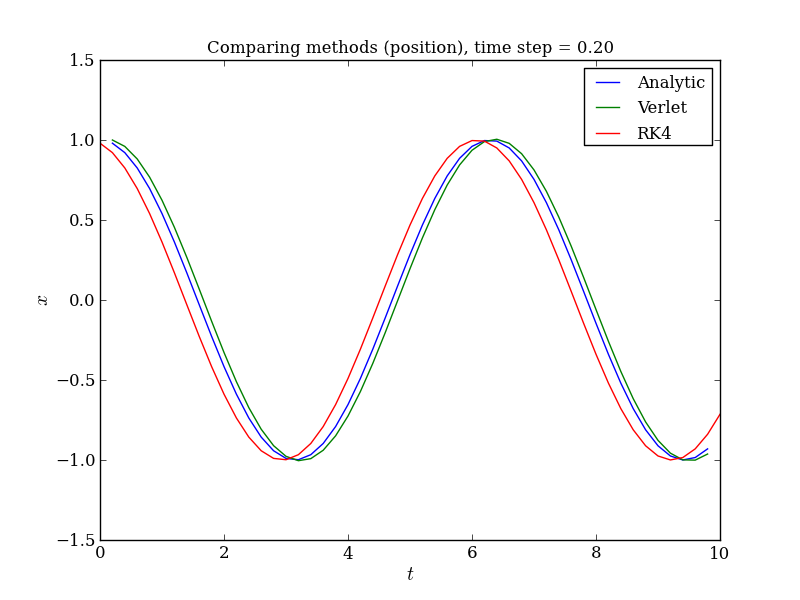
\includegraphics[width=90mm]{Images/comparison_x.png}
	& 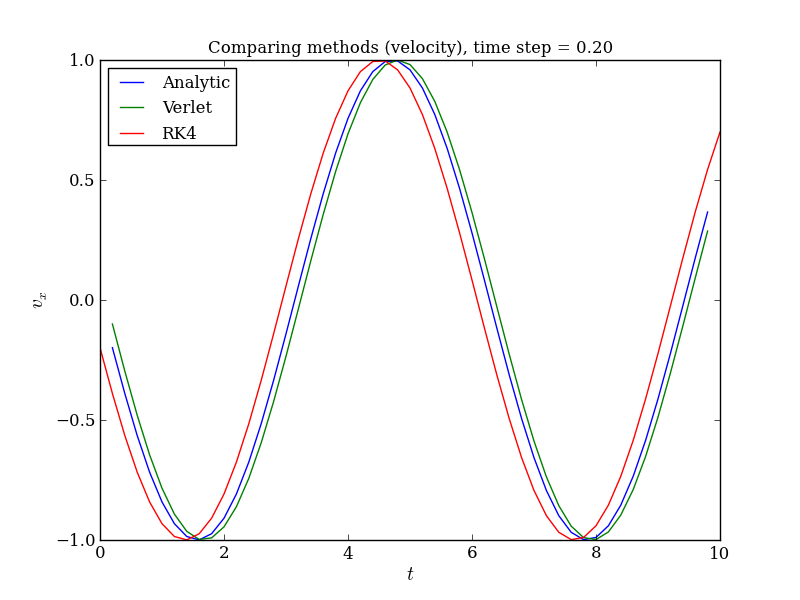
\includegraphics[width=90mm]{Images/comparison_v.png} \\
	(a) Position				& (b) Velocity  \\[6pt]
\end{tabular}
\caption{Comparison of our numerical algorithms, Velocity-Verlet (green) and 4th-order Runge-Kutta (red), with the analytical solution (blue) in the case of the box on a spring. Here for a time step of $\Delta t = 0.2$.}\label{fig:analytical}
\end{center}
\end{figure*}

\noindent Another test we can make is to check for \textbf{energy conservation}. With initial conditions $x_0$ and $v_0$, we can calculate

\begin{equation}
	\begin{aligned}
		E(t = 0) = E_0 &= \frac{1}{2}mv_0^2 + \frac{1}{2}kx_0^2, \\
		E(t = t_i) = E_i &= \frac{1}{2}mv_i^2 + \frac{1}{2}kx_i^2,
	\end{aligned}
\end{equation}
and check that $E_0 = E_i$ for every period $T$. It is however easier to just plot $E_i$ as a function of time for the different methods and inspect the result. If the energy is conserved, the plot should be a straight line, as the energy should not change over time. As shown in Fig.~\ref{fig:analytical_energy} this is indeed the case in the analytical case. If we look closely at the $y$-axis we see that this really is the case for all the methods, with the numerical methods deviating from the expected result in the fifth decimal place. \\

\begin{figure*}[t!]
\begin{center}
  	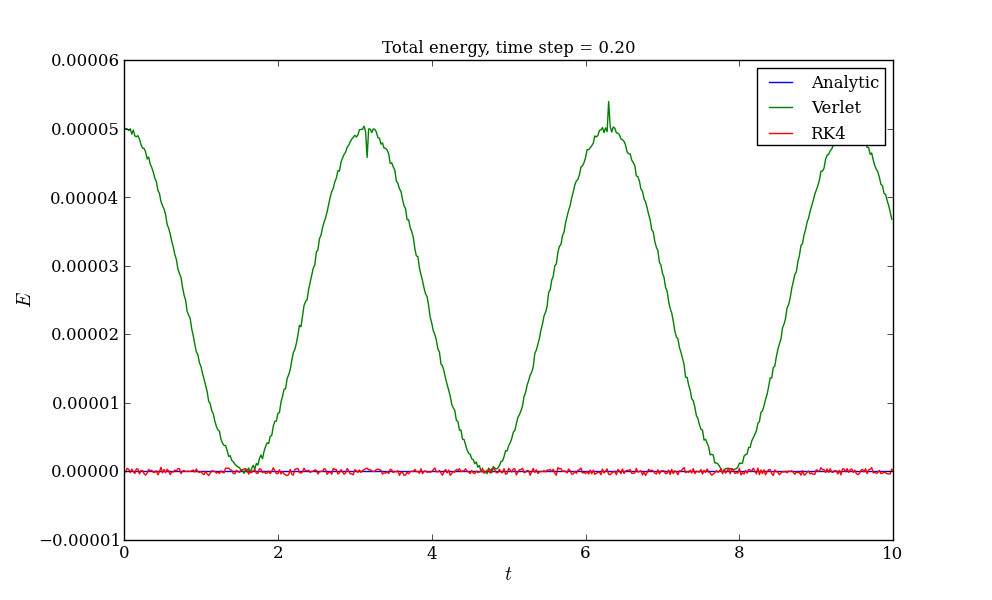
\includegraphics[width=130mm]{Images/energy_conservation.png}
\caption{The total energy $E$ as a function of time $t$ of our numerical algorithms, Velocity-Verlet (green) and 4th-order Runge-Kutta (red), with the analytical solution (blue) in the case of the box on a spring. Here for a time step of $\Delta t = 0.2$.}\label{fig:analytical_energy}
\end{center}
\end{figure*}

\noindent Now that we have verified our numerical methods, we can go on to solve the problem at hand.



\subsection{Stability of methods}

First we consider the Newtonian two-body problem in three dimensions to study the stability of the two methods described in Sec.~\ref{sec:methods}. This is done by running the two algorithms over a very long time period. 

...

We also check how the two methods work for large time steps.
For $h=2$, there is no change in velocity in the case with VV.
...

For very long times, we see that there is a damping in the curve for RK4, but not for VV.
...

What is also interesting is to compare the time used to advance one time step for the two different methods, to see which one is the most efficient.

...

Based on our study of the stability and time usage of the two methods, we can say that ... COMMENT. \\


\noindent We go on to look at the $N$-body system. For a system with $N = 100$ and a radius $R_0$ = 20 ly, a time step of XXXX is required.

We run the calculations for both methods in Sec.~\ref{sec:methods}. XXX





\section{Conclusions}

...




\section{List of codes}

The codes developed and used in this project are: 


\subsection{Running calculations (C++)}

\begin{itemize}
	\item \verb@main.cpp@ -- main program where the calculations are run, calling on the classes listed below. 
	\item \verb@solver.cpp@ -- class containing the numerical methods.
	\item \verb@star.cpp@ -- class collecting various properties of the stars.
	\item \verb@galaxy.cpp@ -- class containing all the stars in the galaxy.
\end{itemize}


\subsection{Plotting (Python)}

\begin{itemize}
	\item \verb@plotting_analytical.py@ -- program to graphically compare the one-dimensional 2-body problem with an analytical solution, described in Sec.~\ref{sec:analytical_test}.
	\item \verb@plot_method.py@ -- program to graphically compare the two numerical methods described in Sec.~\ref{sec:RK4} and Sec.~\ref{sec:VV}.
	\item \verb@plotting_scatter.py@ -- plotting program to visualize the $N$-body system in 3D. 
	\item \verb@plotting_radialprofile.py@ -- plotting program that calculates the radial profile of the system, fitted with the profiles in Eq. (\ref{eq:simple_fit}) and Eq. (\ref{eq:NFW}).
\end{itemize}

%\end{multicols}





\clearpage
\appendix
%\onecolumn 
 
\section{Appendix}

\subsection{Nondimensionalization}\label{sec:nondim_deriv}

...



\subsection{Derivation of $t_{\mathrm{crunch}}$}\label{sec:t_crunch_derive}
 
...
 
\subsection{Rewriting of $t_{\mathrm{crunch}}$}\label{sec:G_derive}

We want to write $G$ in units of $\tau_{\mathrm{crunch}}$ so that $G$ becomes a function of the number of particles $N$ and the average mass of the particles $\mu$. Inverting Eq. (\ref{eq:t_crunch}) with respect to $G$, gives

\begin{equation}\label{eq:G}
	G = \frac{3\pi}{32 \rho_0} \frac{1}{\tau_{\mathrm{crunch}}^2},
\end{equation}
where we can replace $\rho_0$ by using that

\begin{equation}
	\mu = \frac{\bar{M}}{M_{\odot}} = \frac{\rho_0}{N M_{\odot}} \quad \Rightarrow \quad \rho_0 = \mu N M_{\odot},
\end{equation}
where $N$ is the total number of particles and $\bar{M}$ is the average mass of the system. Then we can rewrite Eq. (\ref{eq:G}) as 

\begin{equation}
	G = \frac{3\pi}{32 \mu N M_{\odot}} \frac{1}{\tau_{\mathrm{crunch}}^2}.
\end{equation}


\end{multicols}

\end{document}
